\documentclass[10pt]{beamer}

\usetheme{metropolis}
\usepackage{appendixnumberbeamer}

\usepackage{booktabs}
\usepackage[scale=2]{ccicons}

\usepackage{pgfplots}
\usepgfplotslibrary{dateplot}

\usepackage{gb4e}

\usepackage{xspace}
\newcommand{\themename}{\textbf{\textsc{metropolis}}\xspace}
\graphicspath{{figs/}}

\title{The Minimalist Machine}
\subtitle{Some Persian Examples}
\date{April 8, 2016}
\author{Trevor Sullivan \\
Joint work with Sandiway Fong}
\institute{University of Arizona}
% \titlegraphic{\hfill\includegraphics[height=1.5cm]{logo.pdf}}

\begin{document} 

\maketitle

\begin{frame}{Table of contents}
  \setbeamertemplate{section in toc}[sections numbered]
  \tableofcontents[hideallsubsections]
\end{frame}

\section{Introduction to Minimalism}


\begin{frame}[fragile]{Minimalism}
  The diverse grammars for different languages are considered too complicated to be learnable in the very short amount of time that children learn them. 

  The hypothesis of Universal Grammar, the idea that the core of grammatical systems exists in human brains independent of particular language, demands a better solution. 

  In the 80s and 90s there came a push to reconcile all of the wildly different grammars that exist for various languages. 

  \emph{Minimize} the complexity of grammar to a small number of systems that are plausibly innate

\end{frame}

\begin{frame}[fragile]{Minimalism}
  \begin{itemize}[<+->]
    \item Throwing out:
    \begin{itemize}[<+->]
      \item X-bar
      \item Government + Binding
    \end{itemize}
    \item New concepts:
    \begin{itemize}[<+->]
      \item Bare Phrase Structure
      \item Phases CP and sometimes vP
      
        (Nothing can move out of a phase unless it is at the left edge of that phase)
      
      \item Interpretation through valuation of features
    \end{itemize}
  \end{itemize}
\end{frame}


\begin{frame}[fragile]{Feature Valuation}
  \begin{description}[Uninterpretable Features]
    \item[Interpretable Features] Information that is contained within a head and can be read by other heads. 
      
      eg: plurality in ``cats'' and tense on ``did''
    \item[Uninterpretable Features] Features present on a head that have no information of their own \emph{until} they are matched with an interpretable feature. uFs are deleted at the Conceptual-Intensional interface, if valued. 

    \item[Edge Features] Feature that is satisfied when an item merges into the head's left edge (spec) position. There is debate over whether Edge Features are their own category, or a subtype of uF. 
  \end{description}
  Uninterpretable feature and edge feature valuation is performed by an action called ``agree'' through a ``probe-goal'' mechanism that reaches down into the tree.
\end{frame}




\begin{frame}[fragile]{Theory note}
  The minimalist program is not without critics or faults.
  \pause
  
  \begin{enumerate}[<+->]
    \item No empirical evidence.

    There is no scientific evidence that motivates the existence of the minimalist program, it is not more descriptively powerful than traditional grammars, but it is more theoretically ``perfect''.
    \item Very vague.

    Most discussions of the Minimalist Program do not go deep into the details. For most writers, the question of whether it could work in theory is more important than an investigation of whether it does. 
  \end{enumerate}


\end{frame}


% \section*{What's all this business about a machine?}

\section{The Minimalist Machine}


\begin{frame}[fragile]{The Machine}
  The minimalist machine is a program that constructs derivations according to the minimalist program.\footnote{Based primarily on Chomsky(2001): Derivation by Phase}
  \pause

  In other words, it builds sentences in the same way that brains do.*
  \pause

  An attempt to prove the viability of the Minimalist Program as the core component of UG. It is a mathematical model of what the human language faculty has to compute. 


\end{frame}


\begin{frame}[fragile]{How does it work?}

  \begin{itemize}[<+->]
    \item Prolog
    \item Two parts:
    \begin{enumerate}[<+->]
      \item Universal Grammar
      \begin{itemize}[<+->]
        \item Merge
        \item Agree
      \end{itemize}
      \item Language-Specific Grammar
      \begin{itemize}[<+->]
        \item Lexicon
        \item Features
      \end{itemize}
    \end{enumerate}
  \end{itemize}

\end{frame}




\begin{frame}[fragile]{Derivation Process}
  \pause
  Input Stream
  \begin{itemize}[<+->]
    \item List of heads in reverse order of their merge.
  \end{itemize}
  Stack
  \begin{itemize}[<+->]
    \item Stack (CS Data Structure) of constituents with unvalued features.
    \item Representative of probe-goal.
  \end{itemize}
  Syntactic Object (SO)
  \begin{itemize}[<+->]
    \item Built up over time by merging the existing SO with stream heads or stack constituents.
  \end{itemize}


\end{frame}


\begin{frame}[fragile]{Post Derivation}
  \pause
  \begin{enumerate}[<+->]
    \item Morpheme Realization
    \begin{itemize}[<+->]
      \item Each head in the derivation is spelled out according to rules set in the language-specific grammar.
    \end{itemize}
    \item Affix Hopping
    \begin{itemize}[<+->]
      \item Suffixes hop over the word immediately to their right.
    \end{itemize}
    \item Morpheme Realization part 2
    \begin{itemize}[<+->]
      \item Affixes join with heads.
    \end{itemize}
  \end{enumerate}

\end{frame}






% \section*{Wait a minute, isn't this talk supposed to be about Persian?}

\section{Persian 1:01}

\begin{frame}[fragile]{Persian 1:01}
\only<-3>{  Persian is an Iranian language spoken in Iran, Afghanistan, and Tajikistan.
  \pause

  The written dialect/style is different from the spoken dialect/style. The difference is primarily in pronunciation, which does not matter for us, but where there is a grammatical difference, the spoken form is preferred.
  \pause}

  SOV word order...
  \pause

  Unlike most SOV languages, Persian has prepositions rather than to postpositions, determiners that precede nouns, and complementizers before their related clauses. 
  \pause

  Therefore, we can assert with confidence, as many have, that Persian is a left-headed language in all parameters except the verbal structure. 

  \centerline{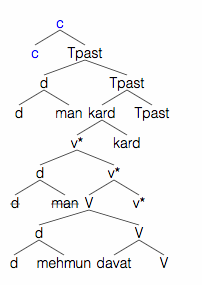
\includegraphics[height=5cm]{headedness.png}}


\end{frame}



\section{Persian Challenges to the Minimalist Program}

\begin{frame}[fragile]{Complex Predicate}
  In Persian, many verbal concepts are expressed not through verbs, but rather through the combination of a non-verb and a semantically bleached light verb. These are henceforth referred to as ``NVE'' and ``LV''.
  \pause
  \begin{exe}
    \ex
    \gll man mehmun davat kardam\\
    1.SG guest invitation do.PST-1.SG\\
    \trans `I invited a guest'
    \trans lit. `I did invitation a guest'
  \end{exe}
    \begin{exe}
    \ex
    \gll Bahar zabun yâd gereft-Ø\\
    B. language memory take.PST-3.SG\\
    \trans `Bahar learned a language'
    \trans lit. `Bahar took memory a language'
  \end{exe}

  \pause

  Complex Predicates are often idiomatic in meaning, but not in nature: they take an object, can be separated by adverbs (sometimes), can be transitive or intransitive (ie, the NVE is \emph{not} a direct object).

\end{frame}

\begin{frame}[fragile]{Complex Predicate}
  % talk a bit about what doesn't work first
  \textbf{Solution: }\pause Build in a pre-narrow-syntax morphology. \pause

  Add to the Persian Grammar module a verbalizer. The verbalizer attaches to a non-verbal head, and the resulting SO is \emph{not} a constituent, but rather, remains a head. 
  \pause

  \only<4>{\centerline{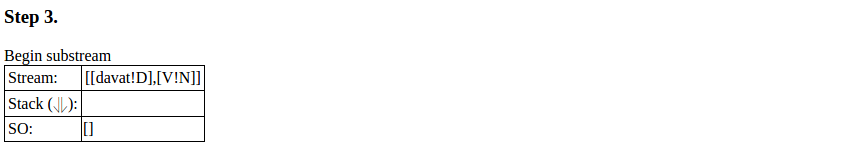
\includegraphics[width=10cm]{verbalizer1.png}}}
  \only<5>{\centerline{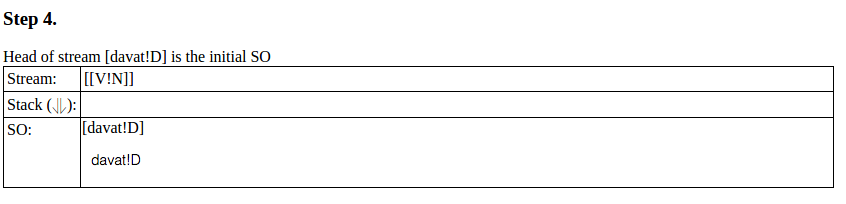
\includegraphics[width=10cm]{verbalizer2.png}}}
  \only<6>{\centerline{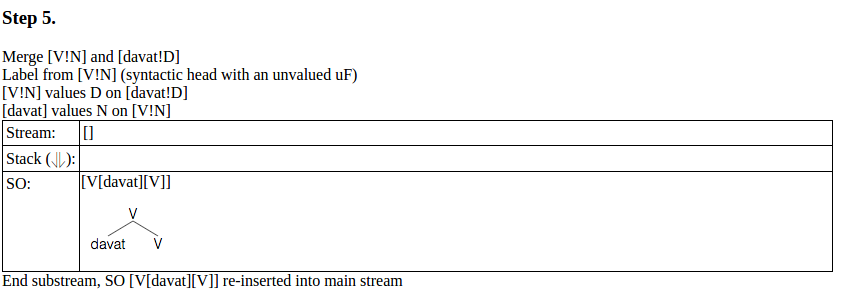
\includegraphics[width=10cm]{verbalizer3.png}}}
  \only<7>{\centerline{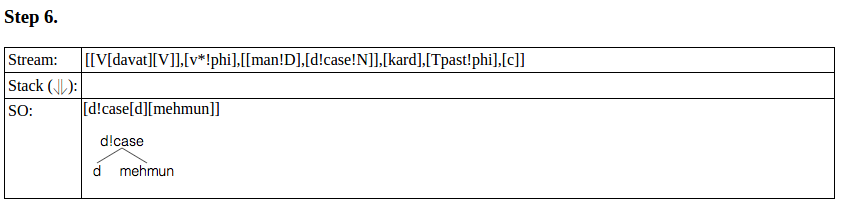
\includegraphics[width=10cm]{verbalizer4.png}}}
  \only<8->{\centerline{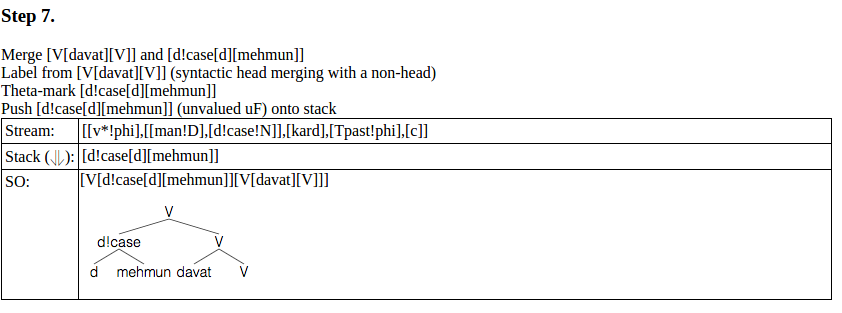
\includegraphics[width=10cm]{verbalizer5.png}}}


  \only<9->{  This kind of operation is not precedented as part of narrow syntax, but syntacticians often assume that certain morphological operations can take place before narrow syntax. }    


\end{frame}



\begin{frame}[fragile]{Complex Predicate}
  \textbf{What about LV?} \pause

  Scholarly consensus is that the light verb in Complex Predicate is a v. That is uncontested here.

  Many LVs are possible, more than the traditional count of little vs, and they serve some semantic purpose, whereas v is purely functional, eg

  \begin{columns}
    \column{.5\textwidth}
      \begin{exe}
        \ex
        \gll yâd gereftan\\
        memory taking\\
        \trans `learn'
      \end{exe}

      is semantically distinct from

      \begin{exe}
        \ex
        \gll yâd âvardan\\
        memory getting\\
        \trans `remember'
      \end{exe}

    \column{.5\textwidth}
      whereas
      \begin{exe}
         \ex
        \gll (v*) eat steak\\
        . .\\
      \end{exe}
      
      has the same semantic content as

      \begin{exe}
         \ex
        \gll steak (v\~) eaten\\
        . .\\
      \end{exe}
  \end{columns}

  v can move arguments, but not change the core semantics of a word.

\end{frame}



\begin{frame}[fragile]{Complex Predicate}
  Therefore, we consider v to be distinct from LV, and as a result, the LV is merged to the tree at its own level.

  \only<2>{\centerline{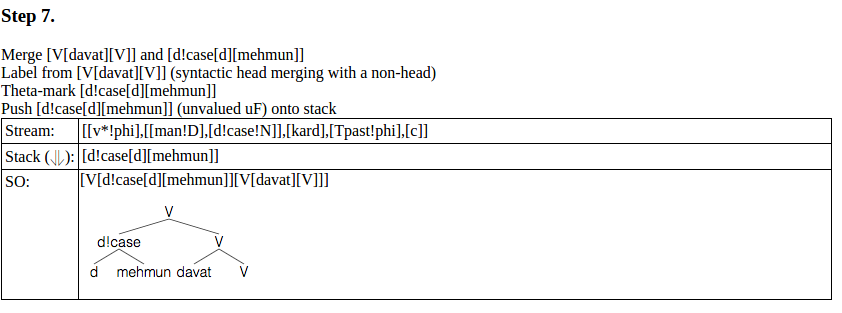
\includegraphics[width=10cm]{verbalizer5.png}}}
  \only<3>{\centerline{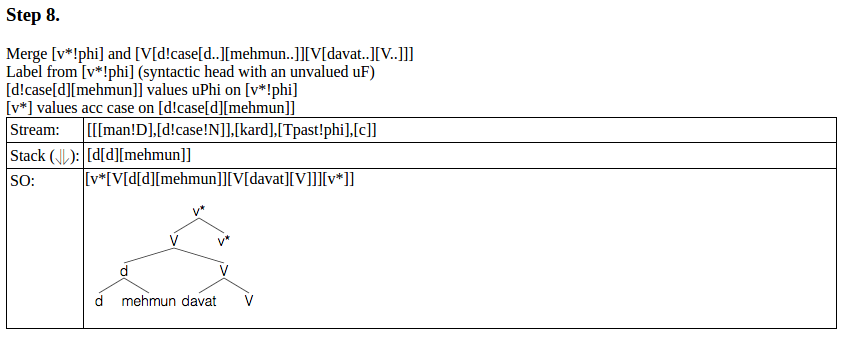
\includegraphics[width=10cm]{verbalizer6.png}}}
  \only<4>{\centerline{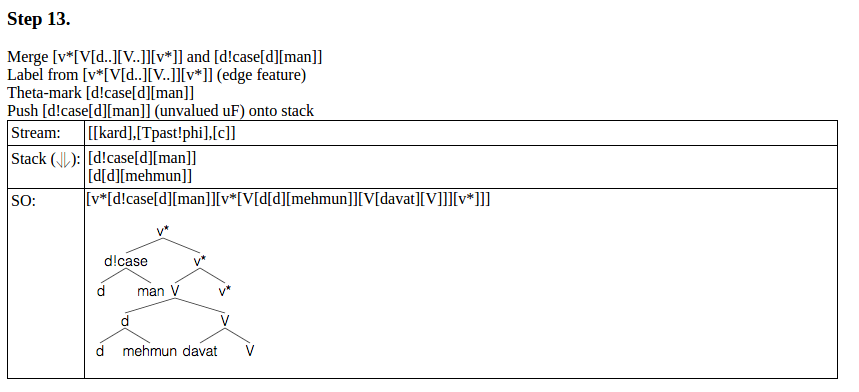
\includegraphics[width=10cm]{verbalizer7.png}}}
  \only<5>{\centerline{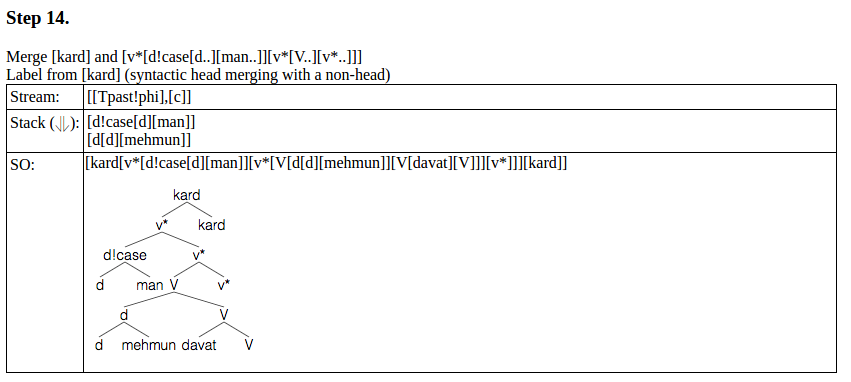
\includegraphics[width=10cm]{verbalizer8.png}}}
  \only<6>{\centerline{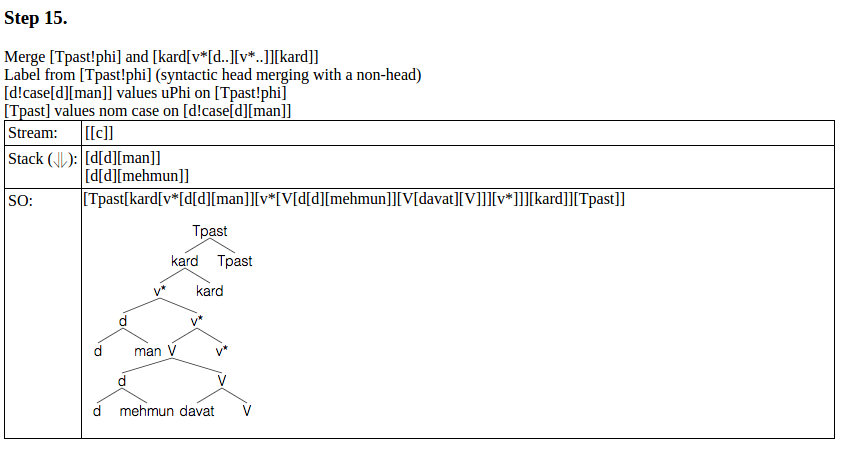
\includegraphics[width=10cm]{verbalizer9.png}}}


\end{frame}

\section*{Verbal Morphology}


\begin{frame}[fragile]{Verbal Morphology}
  \pause
  Since T is right-headed (as it is part of the verbal complex, this is the null hypothesis), it is trivial to get the morphology containing the subject's $\phi$-features and the sentential tense in the right position, but there are three verbal morphemes that are difficult to place in the tree structure. Each of the following are prefixes that attach to the main verb, or light verb in Complex Predicates. 

  \metroset{block=fill}
  \begin{block}{Verbal prefixes}
    \vspace{5mm}
    \begin{columns}[T, onlytextwidth]
      \column{.33\textwidth}
        mi- (durative aspect)
      \column{.33\textwidth}
        na- (negation)
      \column{.33\textwidth}
        be- (subjunctive)
    \end{columns}
  \end{block}
  \pause
  These things appear to represent verbal concepts, and as such we would expect them to be right-headed like the rest of the verbal complex. However, this would put them on the wrong side of the verb to which they attach.

  \pause
  It has been proposed that they are left-headed, but this would require motivating absolutely everything under them, includind NVE to move left past it. 

\end{frame}


\begin{frame}[fragile]{A new definition for Affix Hopping}
  \pause
\only<-3>{  This problem can be solved by making a new definition for affix hopping. }
  \begin{columns}[T,onlytextwidth]
    \column{0.5\textwidth}

    \metroset{block=fill}

      \begin{block}{Head-Initial Phrases}
        \begin{itemize}
          \item Prefixes do not hop.
          \item Suffixes hop.
        \end{itemize}
      \end{block}


    \column{0.5\textwidth}

      \metroset{block=fill}

      \begin{block}{Head-Final Phrases}
        \begin{itemize}
          \item Prefixes hop.
          \item Suffixes do not hop.
        \end{itemize}
      \end{block}

  \end{columns}

  \pause
  This may not be the most theoretically pleasing, since some of the structure from narrow syntax is leaking into the phonological operations post-syntax, but it functions too beautifully to set aside. Furthermore, it makes a testable prediction, something that Minimalism has in short supply.

  \pause
  This is realized in the Machine with a different type of hyphen that the head in question spells out with.


  \begin{columns}[T,onlytextwidth]
    \column{0.5\textwidth}

    \metroset{block=fill}

      \begin{block}{Head-Initial Phrases}
        x\~ - prefix that does not hop \\
        -x - suffix that hops
      \end{block}


    \column{0.5\textwidth}

      \metroset{block=fill}

      \begin{block}{Head-Final Phrases}
        x= - prefix that hops\\
        \#x - suffix that does not hop
      \end{block}

  \end{columns}

\end{frame}


\begin{frame}[fragile]{Affix Hopping Example}
  
  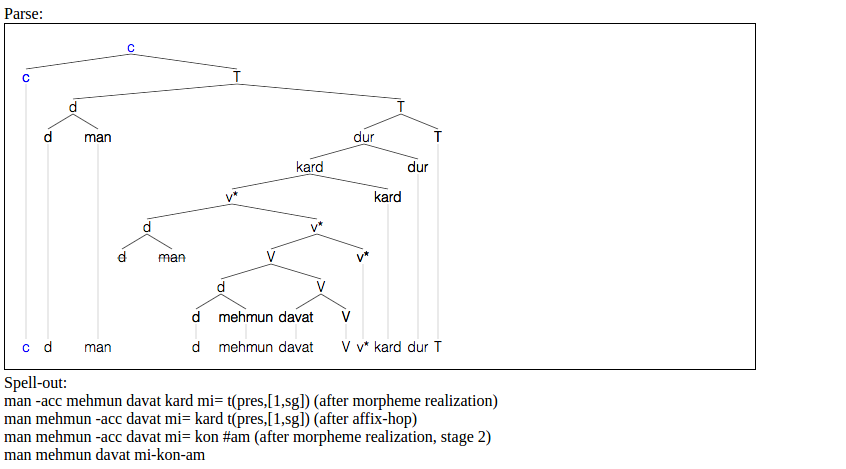
\includegraphics[width=12cm]{affixhopping.png}
  
\end{frame}

\section*{Specific Object Movement}


\begin{frame}[fragile]{Specific Objects}
  Persian has a specificity distinction, but only in direct objects. It is marked with the phrase-level suffix ``-ro'' (``-râ'' in written and formal speech)

  The difference is not only in interpretation, however, because the specific and nonspecific objects have different distributions. 

  \begin{exe}
    \ex
    \gll Bahar diruz miz tamiz kard-Ø\\
    B. yesterday table clean do.PST-3.SG\\
    \trans `Bahar cleaned the table yesterday'
  \end{exe}
  \begin{exe}
    \ex
    \gll Bahar miz-a-ro diruz tamiz kard-Ø\\
    B. table-PL-SPF yesterday clean do.PST-3.SG\\
    \trans `Bahar cleaned the (particular) tables yesterday'
  \end{exe}


\end{frame}

\begin{frame}[fragile]{Specific Objects}
  Furthermore, there is a stark contrast concerning which item can be deleted with the NVE in a complex predicate. 
  \pause
  \begin{exe}
    \ex
    \gll *Bahar miz tamiz kard-Ø, vali Reza pangere kard-Ø\\
    B. table clean do.PST-3.SG but R. window do.PST-3.SG\\
    \trans `Bahar cleaned the table, but Reza did the window'
  \end{exe}
  \only<3>{\begin{exe}
      \ex
      \gll Bahar miz-a-ro tamiz kard-Ø, vali Reza pangere-ha-ro kard-Ø\\
      B. table-PL-SPF clean do.PST-3.SG but R. window-PL-SPF do.PST-3.SG\\
      \trans `Bahar cleaned the (particular) tables, but Reza did the (particular) windows'
    \end{exe}}

  \only<4>{\begin{exe}
      \ex
      \gll Bahar miz-a-ro tamiz kard-Ø, vali pangere-ha-ro na-kard-Ø\\
      B. table-PL-SPF clean do.PST-3.SG but window-PL-SPF NEG-do.PST-3.SG\\
      \trans `Bahar cleaned the (particular) tables, but didn't the (particular) windows'
    \end{exe}}

  
\end{frame}

\begin{frame}[fragile]{Proposed Explanation}
  \pause
\only<-3>{  If it is assumed that prepositional phrases attach to V, the first examples merely require the specific object to move left of V, with no regards to where. }

  \pause
  The second set of ellipsis examples constrains the movement somewhat. At first glance, one is tempted to say that the specific object moves out of vP (or VoiP, if you prefer) \footnote{Karimi,Mahdavi,Nabors,Smith,Sullivan(2016)}, but this presents a problem in minimalism. Firstly, (if one desires the LV to be v or Voi), it requires head movement, which is not allowed in a minimalist framework, but aside from that, it breaks the probe-goal chain. 

  \pause
  \only<4>{\centerline{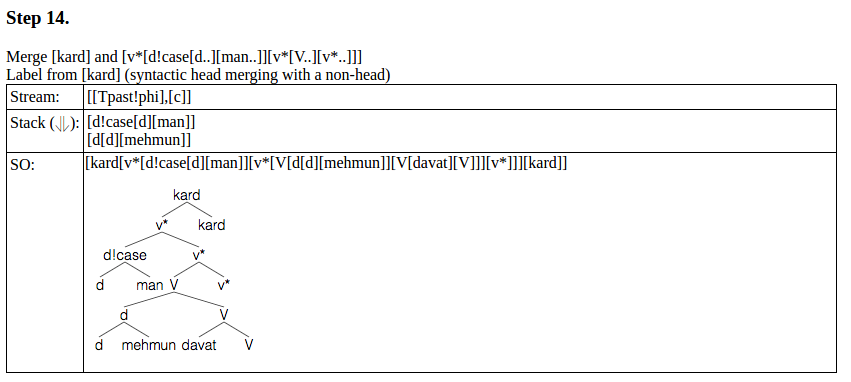
\includegraphics[width=10cm]{verbalizer8.png}}}
  \only<5>{\centerline{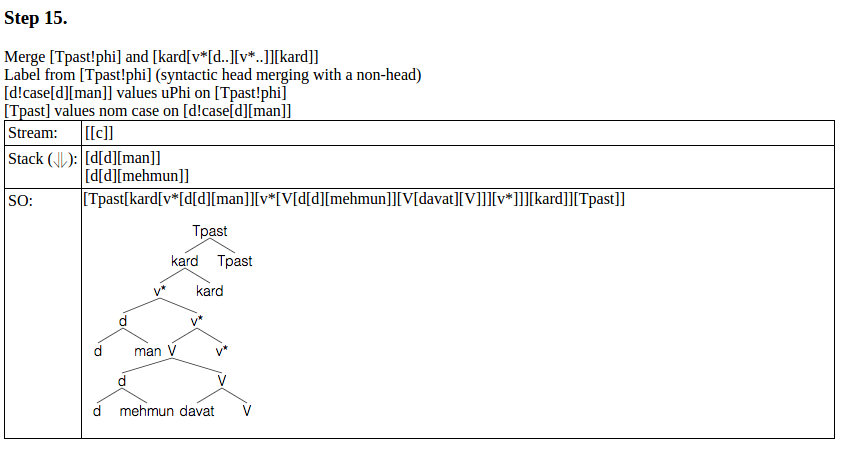
\includegraphics[width=10cm]{verbalizer9.png}}}

  
\end{frame}

\begin{frame}[fragile]{Proposed Explanation}
  \pause
  \only<-6>{It is therefore proposed that the specific object moves to a position below or at v/Voi.\footnote{This has precedent in Karimi(2005)}}

  \pause
  The ellipsis mentioned previously is therefore VP ellipsis, not vP ellipsis. %which I cannot find attestation of anyway

  \pause 
  \begin{exe}
    \ex
    \gll Bahar miz-a-ro tamiz na-kard-Ø, vali pangere-ha-ro kard-Ø\\
    B. table-PL-SPF clean NEG-do.PST-3.SG but window-PL-SPF do.PST-3.SG\\
    \trans `Bahar cleaned the (particular) tables, but didn't the (particular) windows'
  \end{exe}

  \pause
  The subject is a red herring\pause: The observation that it can or cannot be explicitly present in the same ellipsis context implies that it is not part of the ellipsis domain, and is instead a second example NP-ellipsis that happens to co-occur with VP-ellipsis. 


\end{frame}


\begin{frame}[fragile]{Specific Object Movement example}


  \only<1>{\centerline{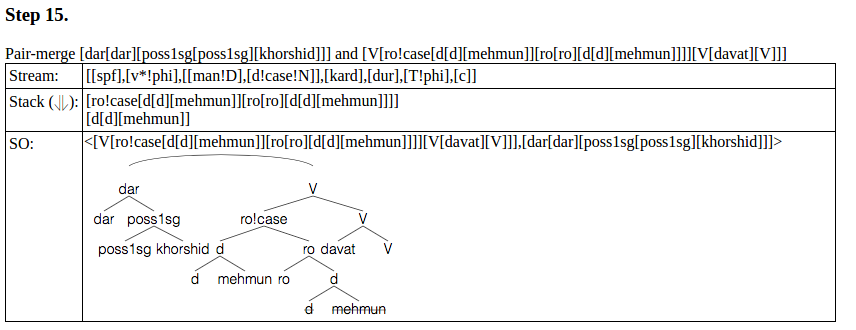
\includegraphics[width=10cm]{ro13.png}}}
  \only<2>{\centerline{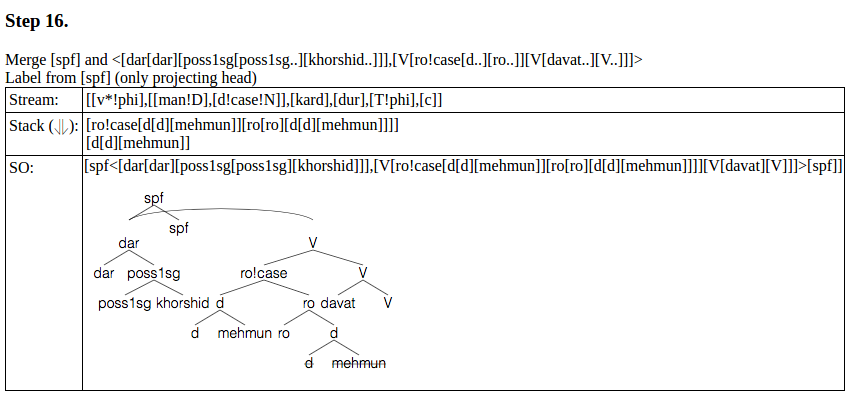
\includegraphics[width=10cm]{ro16.png}}}
  \only<3>{\centerline{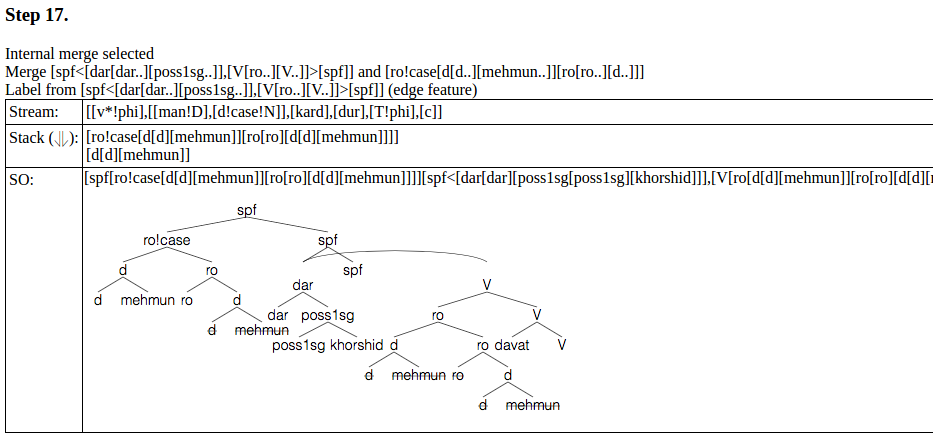
\includegraphics[width=10cm]{ro17.png}}}
  \only<4>{\centerline{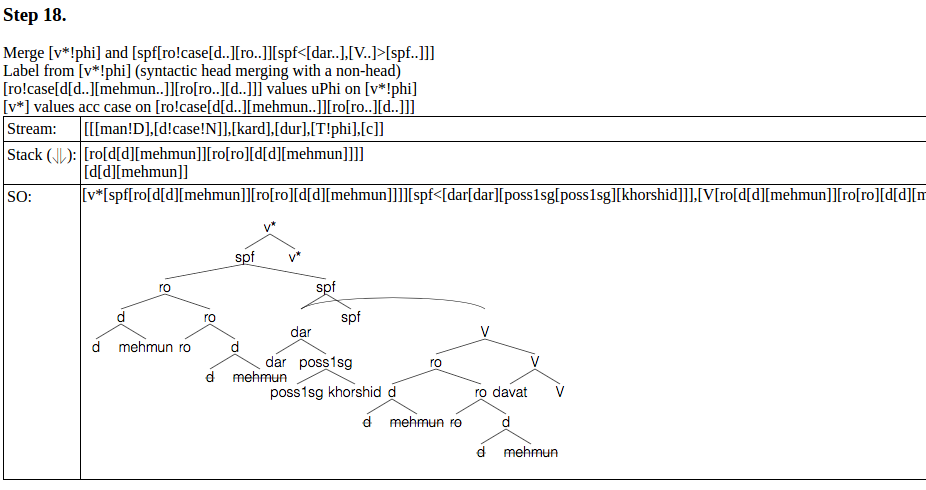
\includegraphics[width=10cm]{ro18.png}}}
  \only<5>{\centerline{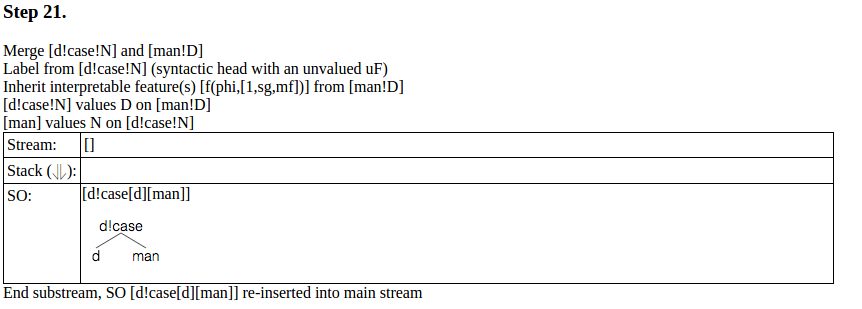
\includegraphics[width=10cm]{ro21.png}}}
  \only<6>{\centerline{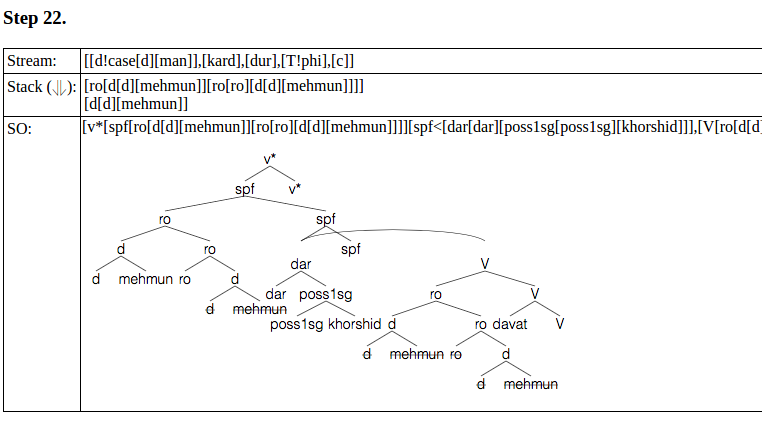
\includegraphics[width=10cm]{ro22.png}}}
  \only<7>{\centerline{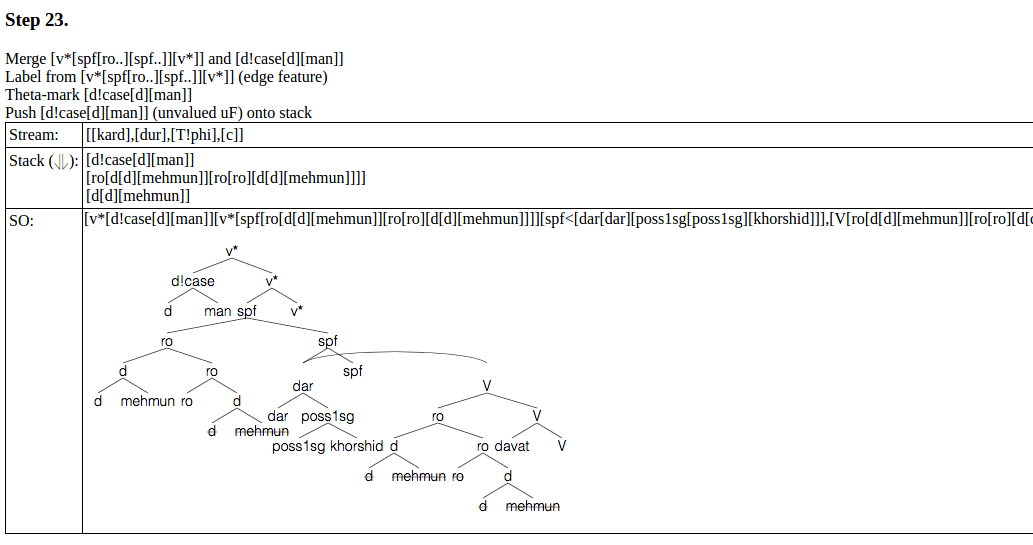
\includegraphics[width=10cm]{ro23.png}}}
  \only<8>{\centerline{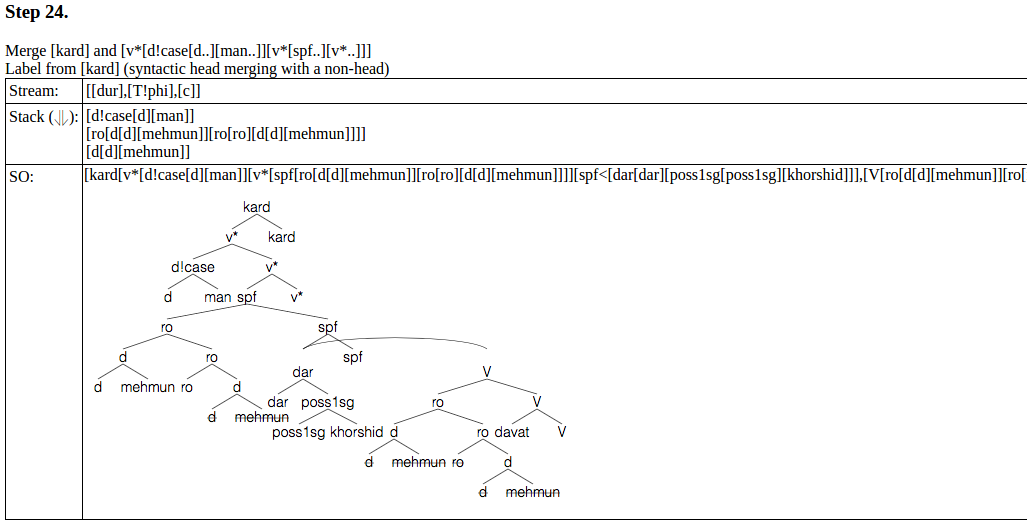
\includegraphics[width=10cm]{ro24.png}}}
  \only<9>{\centerline{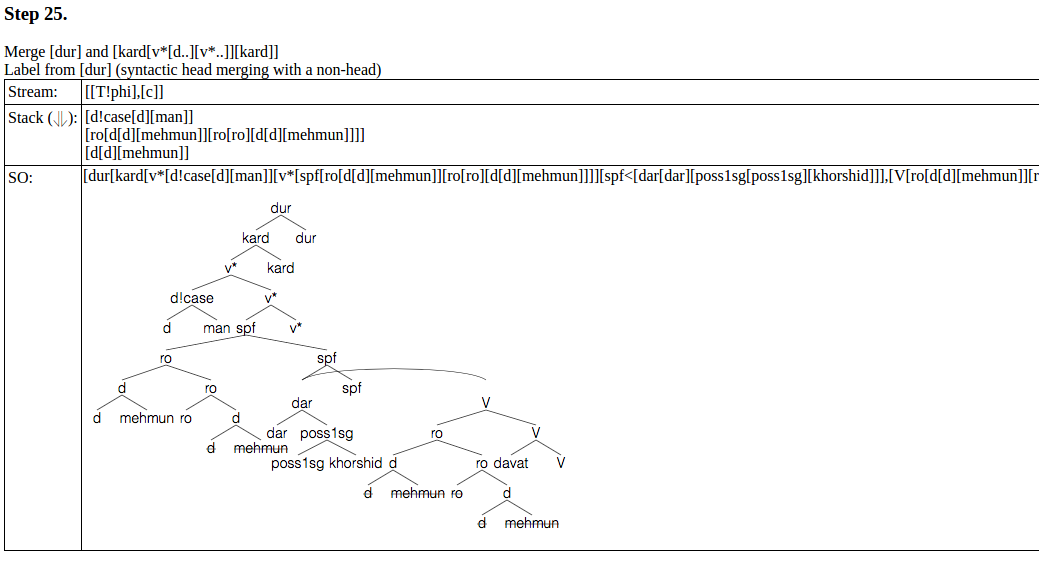
\includegraphics[width=10cm]{ro25.png}}}
  \only<10>{\centerline{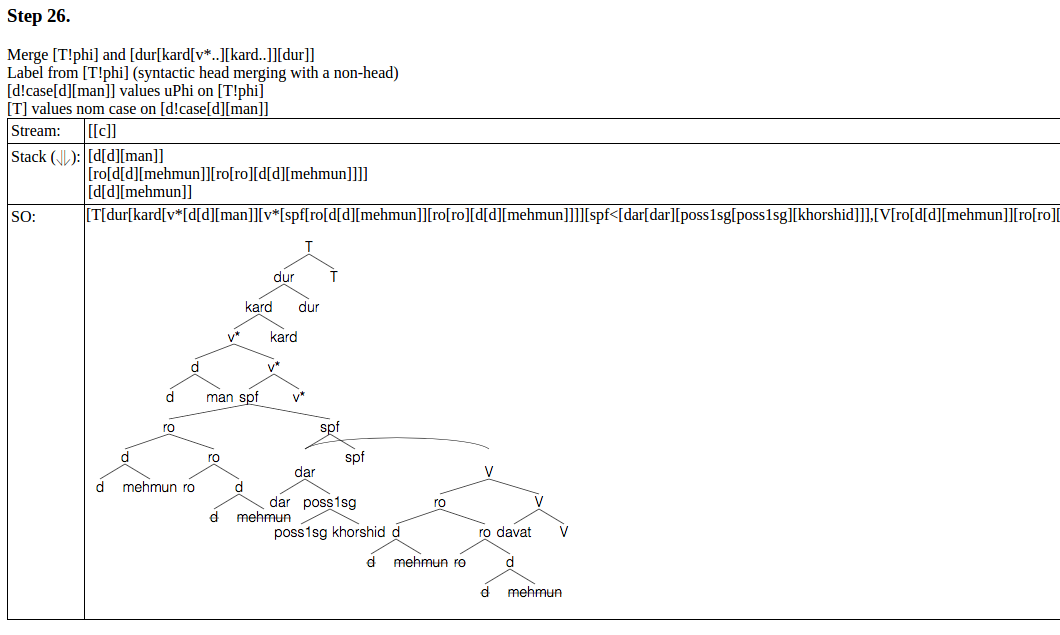
\includegraphics[width=10cm]{ro26.png}}}
  \only<11>{\centerline{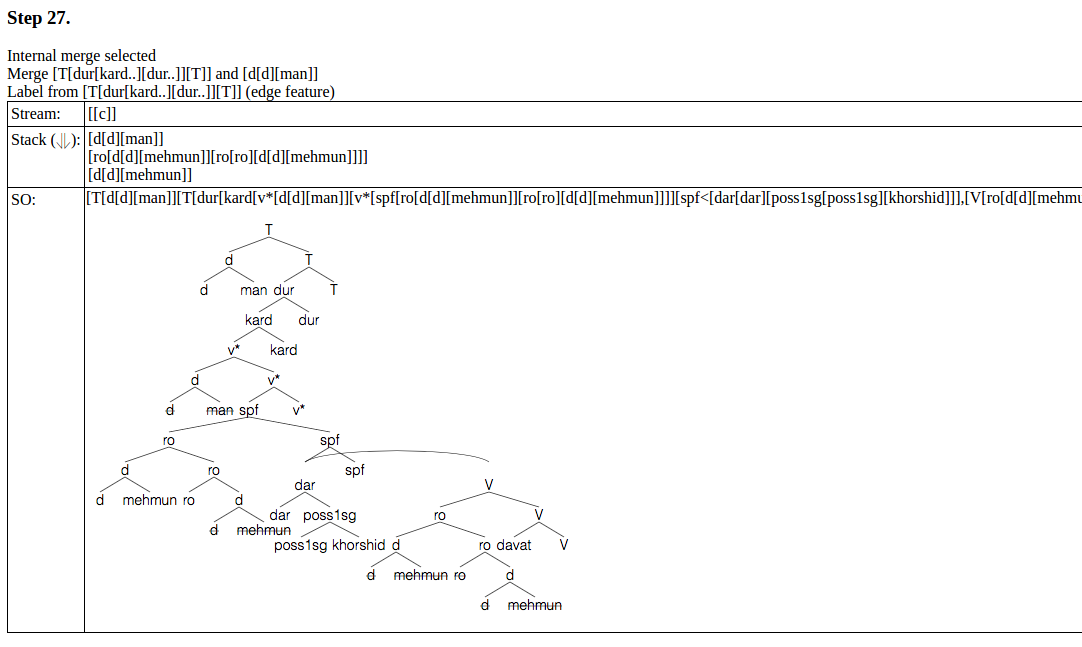
\includegraphics[width=10cm]{ro27.png}}}
  \only<12>{\centerline{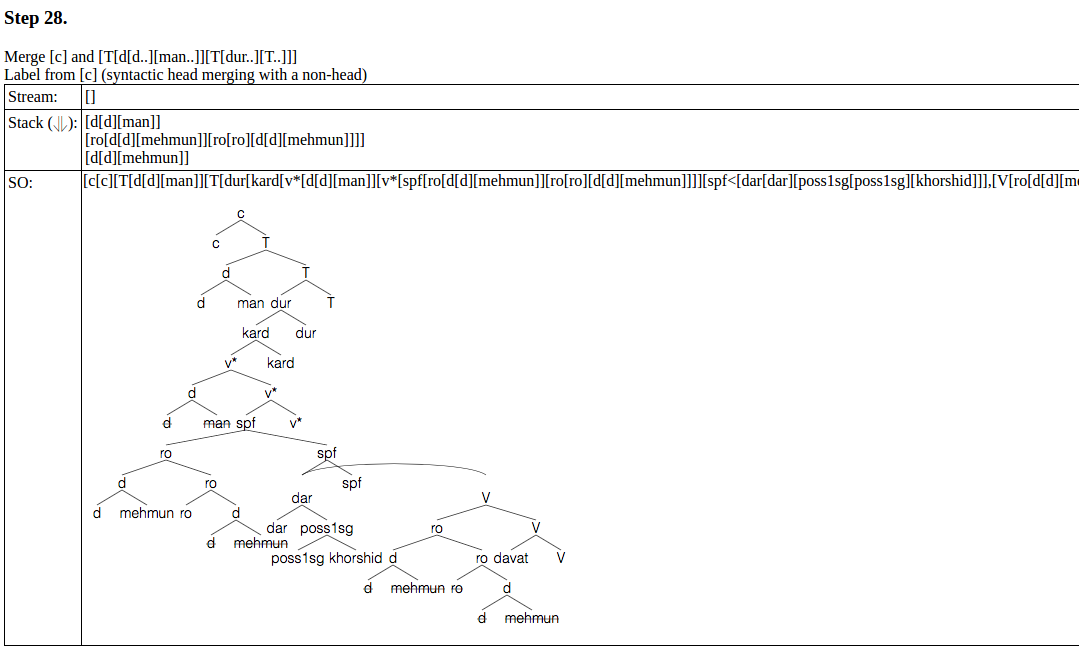
\includegraphics[width=10cm]{ro28.png}}}
  \only<13>{\centerline{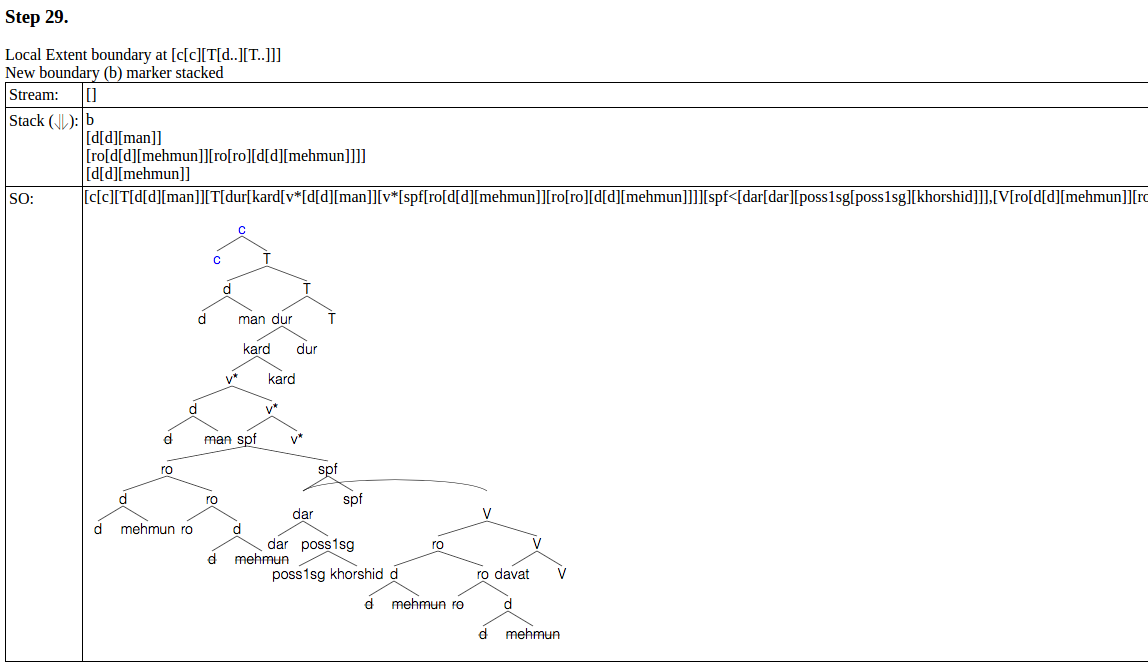
\includegraphics[width=10cm]{ro29.png}}}
  \only<14>{\centerline{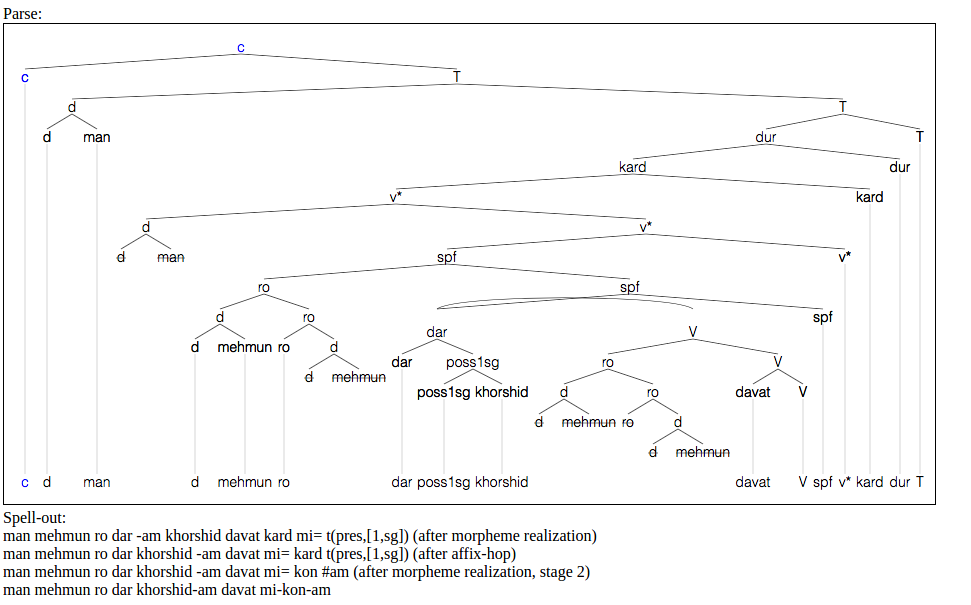
\includegraphics[width=10cm]{rofinal.png}}}

  
\end{frame}





\section{Unsolved Problems with Minimalism and Persian}

\begin{frame}[fragile]{Future Tense}
  \begin{itemize}[<+->]
    \item The Future Tense is marked with what seems to be a verbal object ``khâstan'' that gets the subject's $\phi$-features and appears between the NVE and LV, strongly implying a head-movement relation.
      \begin{exe}
        \ex
        \gll Bahâr miz-â-ro tamiz khâhad-Ø kard\\
        B. table-PL-SPF clean want.PRS-3.SG do.PST\\
        \trans `Bahar will clean the tables'
      \end{exe}
  \end{itemize}
\end{frame}

\begin{frame}[fragile]{Complement Clause Extraposition}
    
  \begin{itemize}[<+->]
    \item Despite being strongly head-final in the verbal complex, Persian internal CPs appear at the end of a sentence. Not only at the end, but after \emph{all} verbal items, including stacked auxiliaries (in dialects that allow them). 
      \begin{exe}
        \ex
        \gll Bahâr goft-Ø ke Reza zabun yâd gereft-Ø\\
        B. say.PST-3.SG that R. language memory take.PST-3SG\\
        \trans `Bahar said that Reza learned the language'
      \end{exe}
    \item This problem also exists in German, and to the best of my knowledge, there is no satisfying solution. 
  \end{itemize}

  
  
\end{frame}



\section{Conclusion}

\begin{frame}{Summary}

  It is possible to build a functional grammar for Persian in a Minimalist Program framework, but it isn't easy.

  Additional allowances for Morphology need to be made in above the pure Minimalist Program.

  A new rule for the spell-out of affixes is proposed, donating a new testable hypothesis to an otherwise not-very-scientific framework. 

  And even then, minimalism not quite good enough to describe every aspect of the language (but still an improvement over willy-nilly phrase-structure grammars, and a worthwhile step forward towards finding UG). 

\end{frame}

\begin{frame}[standout]
  Questions?
\end{frame}

\appendix

\begin{frame}[fragile]{Backup slides}
  % Sometimes, it is useful to add slides at the end of your presentation to
  % refer to during audience questions.

  % The best way to do this is to include the \verb|appendixnumberbeamer|
  % package in your preamble and call \verb|\appendix| before your backup slides.

  % \themename will automatically turn off slide numbering and progress bars for
  % slides in the appendix.
\end{frame}

\begin{frame}[fragile]{English Example}

  \only<2>{\centerline{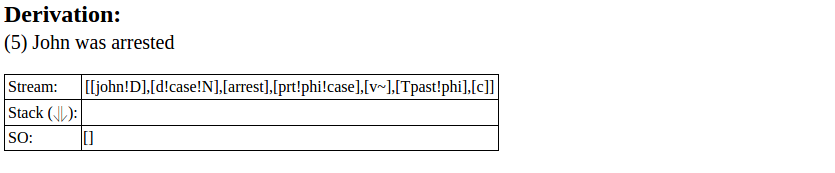
\includegraphics[width=10cm]{eng1.png}}}
  \only<3>{\centerline{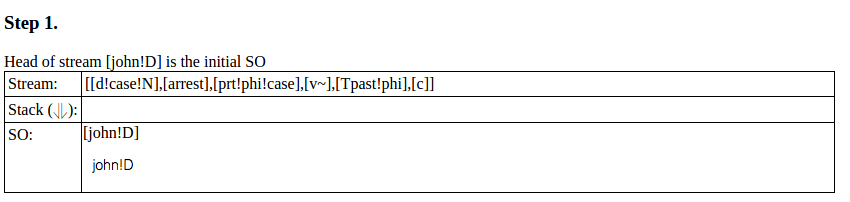
\includegraphics[width=10cm]{eng2.png}}}
  \only<4>{\centerline{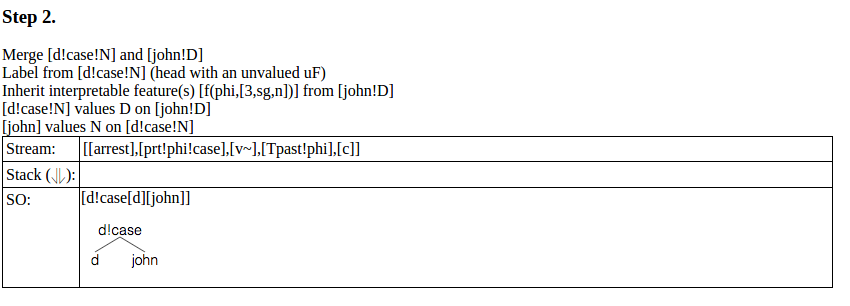
\includegraphics[width=10cm]{eng3.png}}}
  \only<5>{\centerline{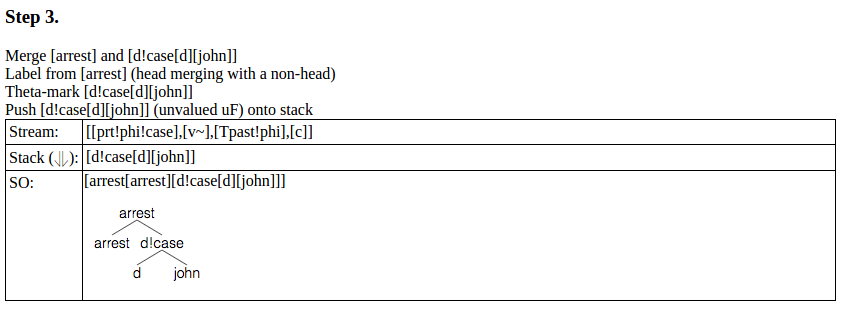
\includegraphics[width=10cm]{eng4.png}}}
  \only<6>{\centerline{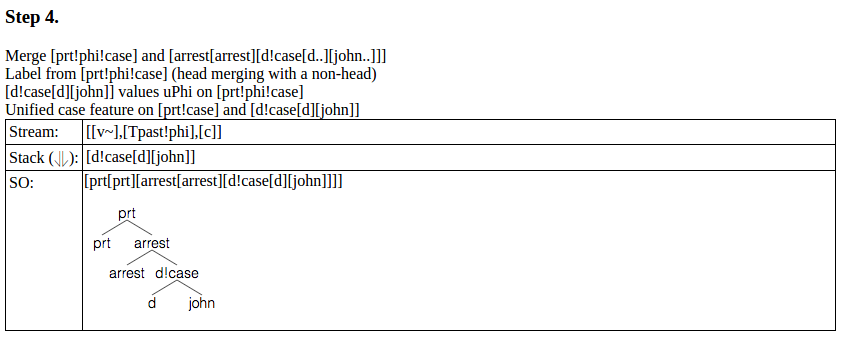
\includegraphics[width=10cm]{eng5.png}}}
  \only<7>{\centerline{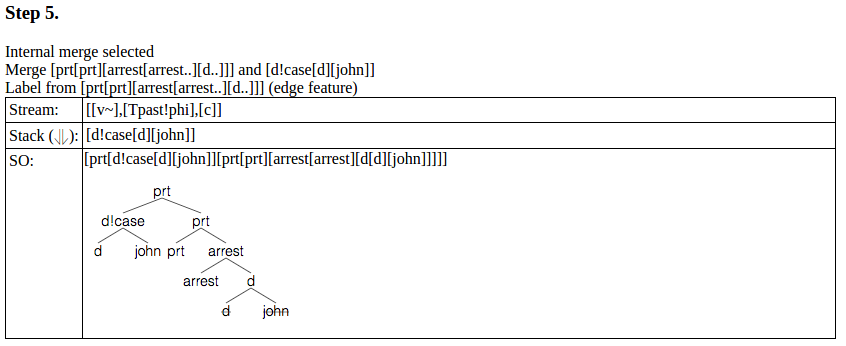
\includegraphics[width=10cm]{eng6.png}}}
  \only<8>{\centerline{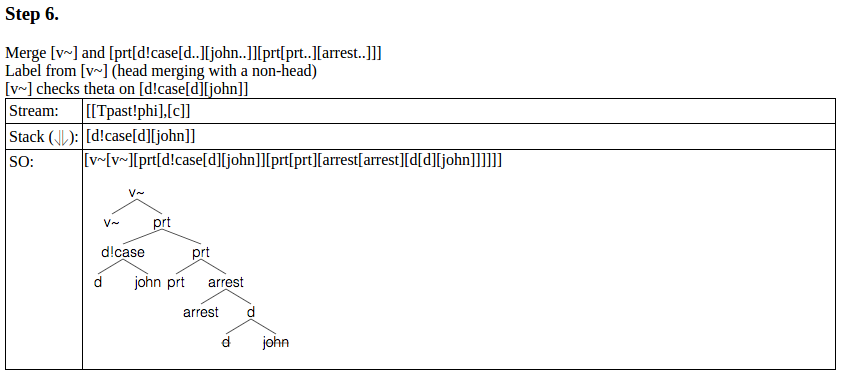
\includegraphics[width=10cm]{eng7.png}}}
  \only<9>{\centerline{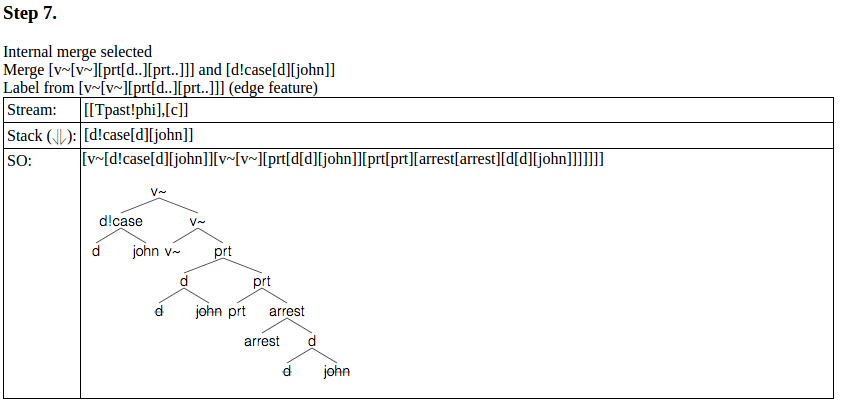
\includegraphics[width=10cm]{eng8.png}}}
  \only<10>{\centerline{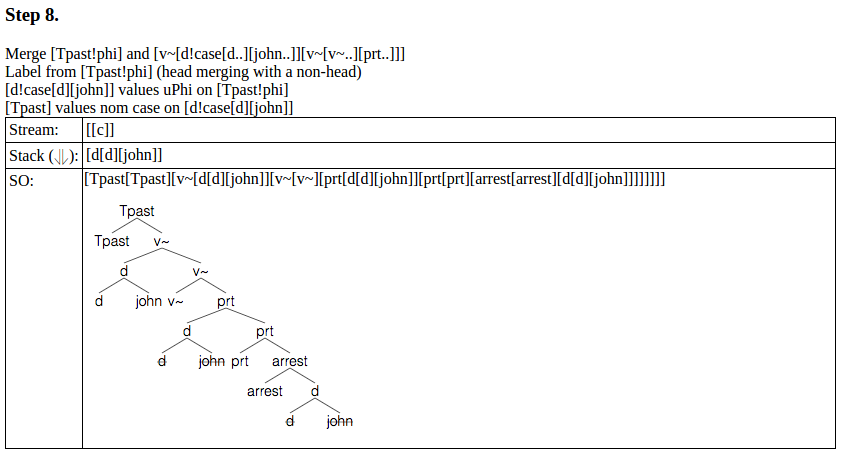
\includegraphics[width=10cm]{eng9.png}}}
  \only<11>{\centerline{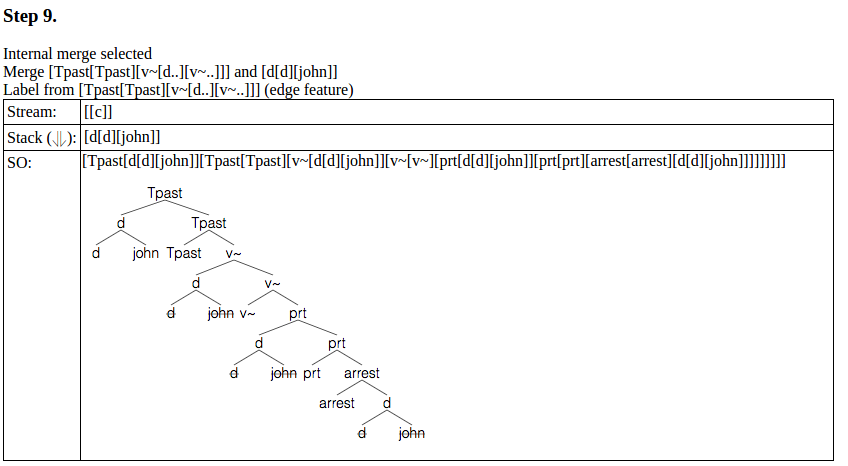
\includegraphics[width=10cm]{eng10.png}}}
  \only<12>{\centerline{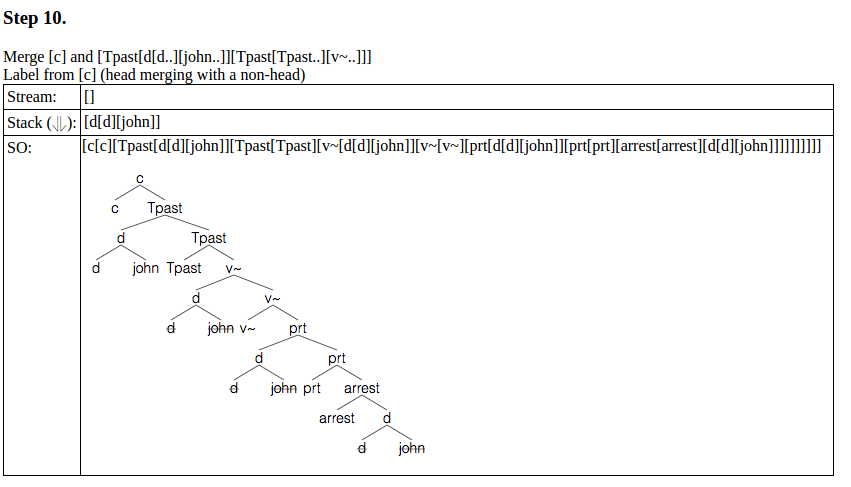
\includegraphics[width=10cm]{eng11.png}}}
  \only<13>{\centerline{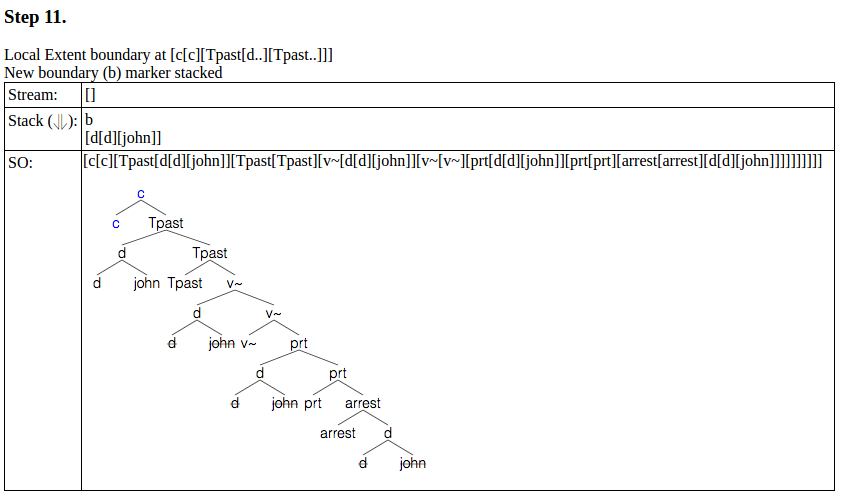
\includegraphics[width=10cm]{eng12.png}}}
  \only<14>{\centerline{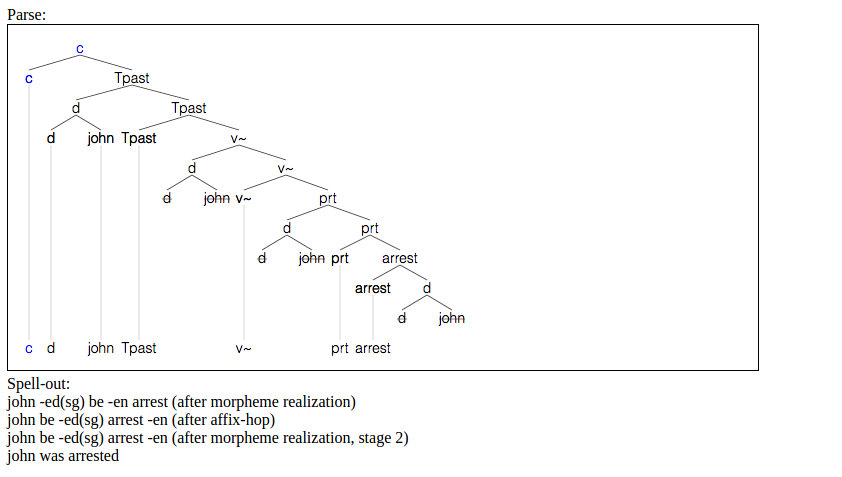
\includegraphics[width=10cm]{eng13.png}}}
  


\end{frame}

\section*{Syntax 1:01}

\begin{frame}[fragile]{Syntax 1:01}
  \begin{itemize}
    \item Language is not linear in nature \pause
    \begin{itemize}[<+->]
      \item \emph{Eagles that fly instinctively swim}
      \item \emph{Instinctively eagles that fly swim}
    \end{itemize}
  \end{itemize}
\end{frame}

\begin{frame}[fragile]{Syntax 1:01}
  \centerline{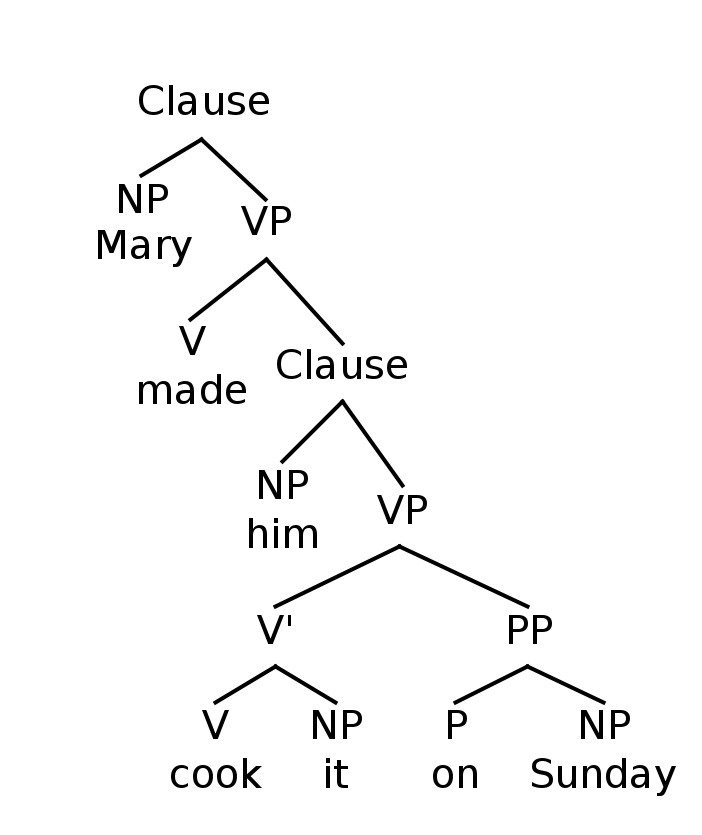
\includegraphics[height=5cm]{marymadehimcookitonsunday.png}} \pause
  \begin{itemize}[<+->]
    \item Binary branching
    \item Phrases and heads
    \item Movement
  \end{itemize}
\end{frame}

\begin{frame}[fragile]{Syntax 1:01}
  
  Does this work for other languages? \pause

  \alert{kinda?}
  
\end{frame}


\begin{frame}[fragile]{Syntax 1:01}
  That John will arrive on time seems to have been considered to be unlikely.

  \centerline{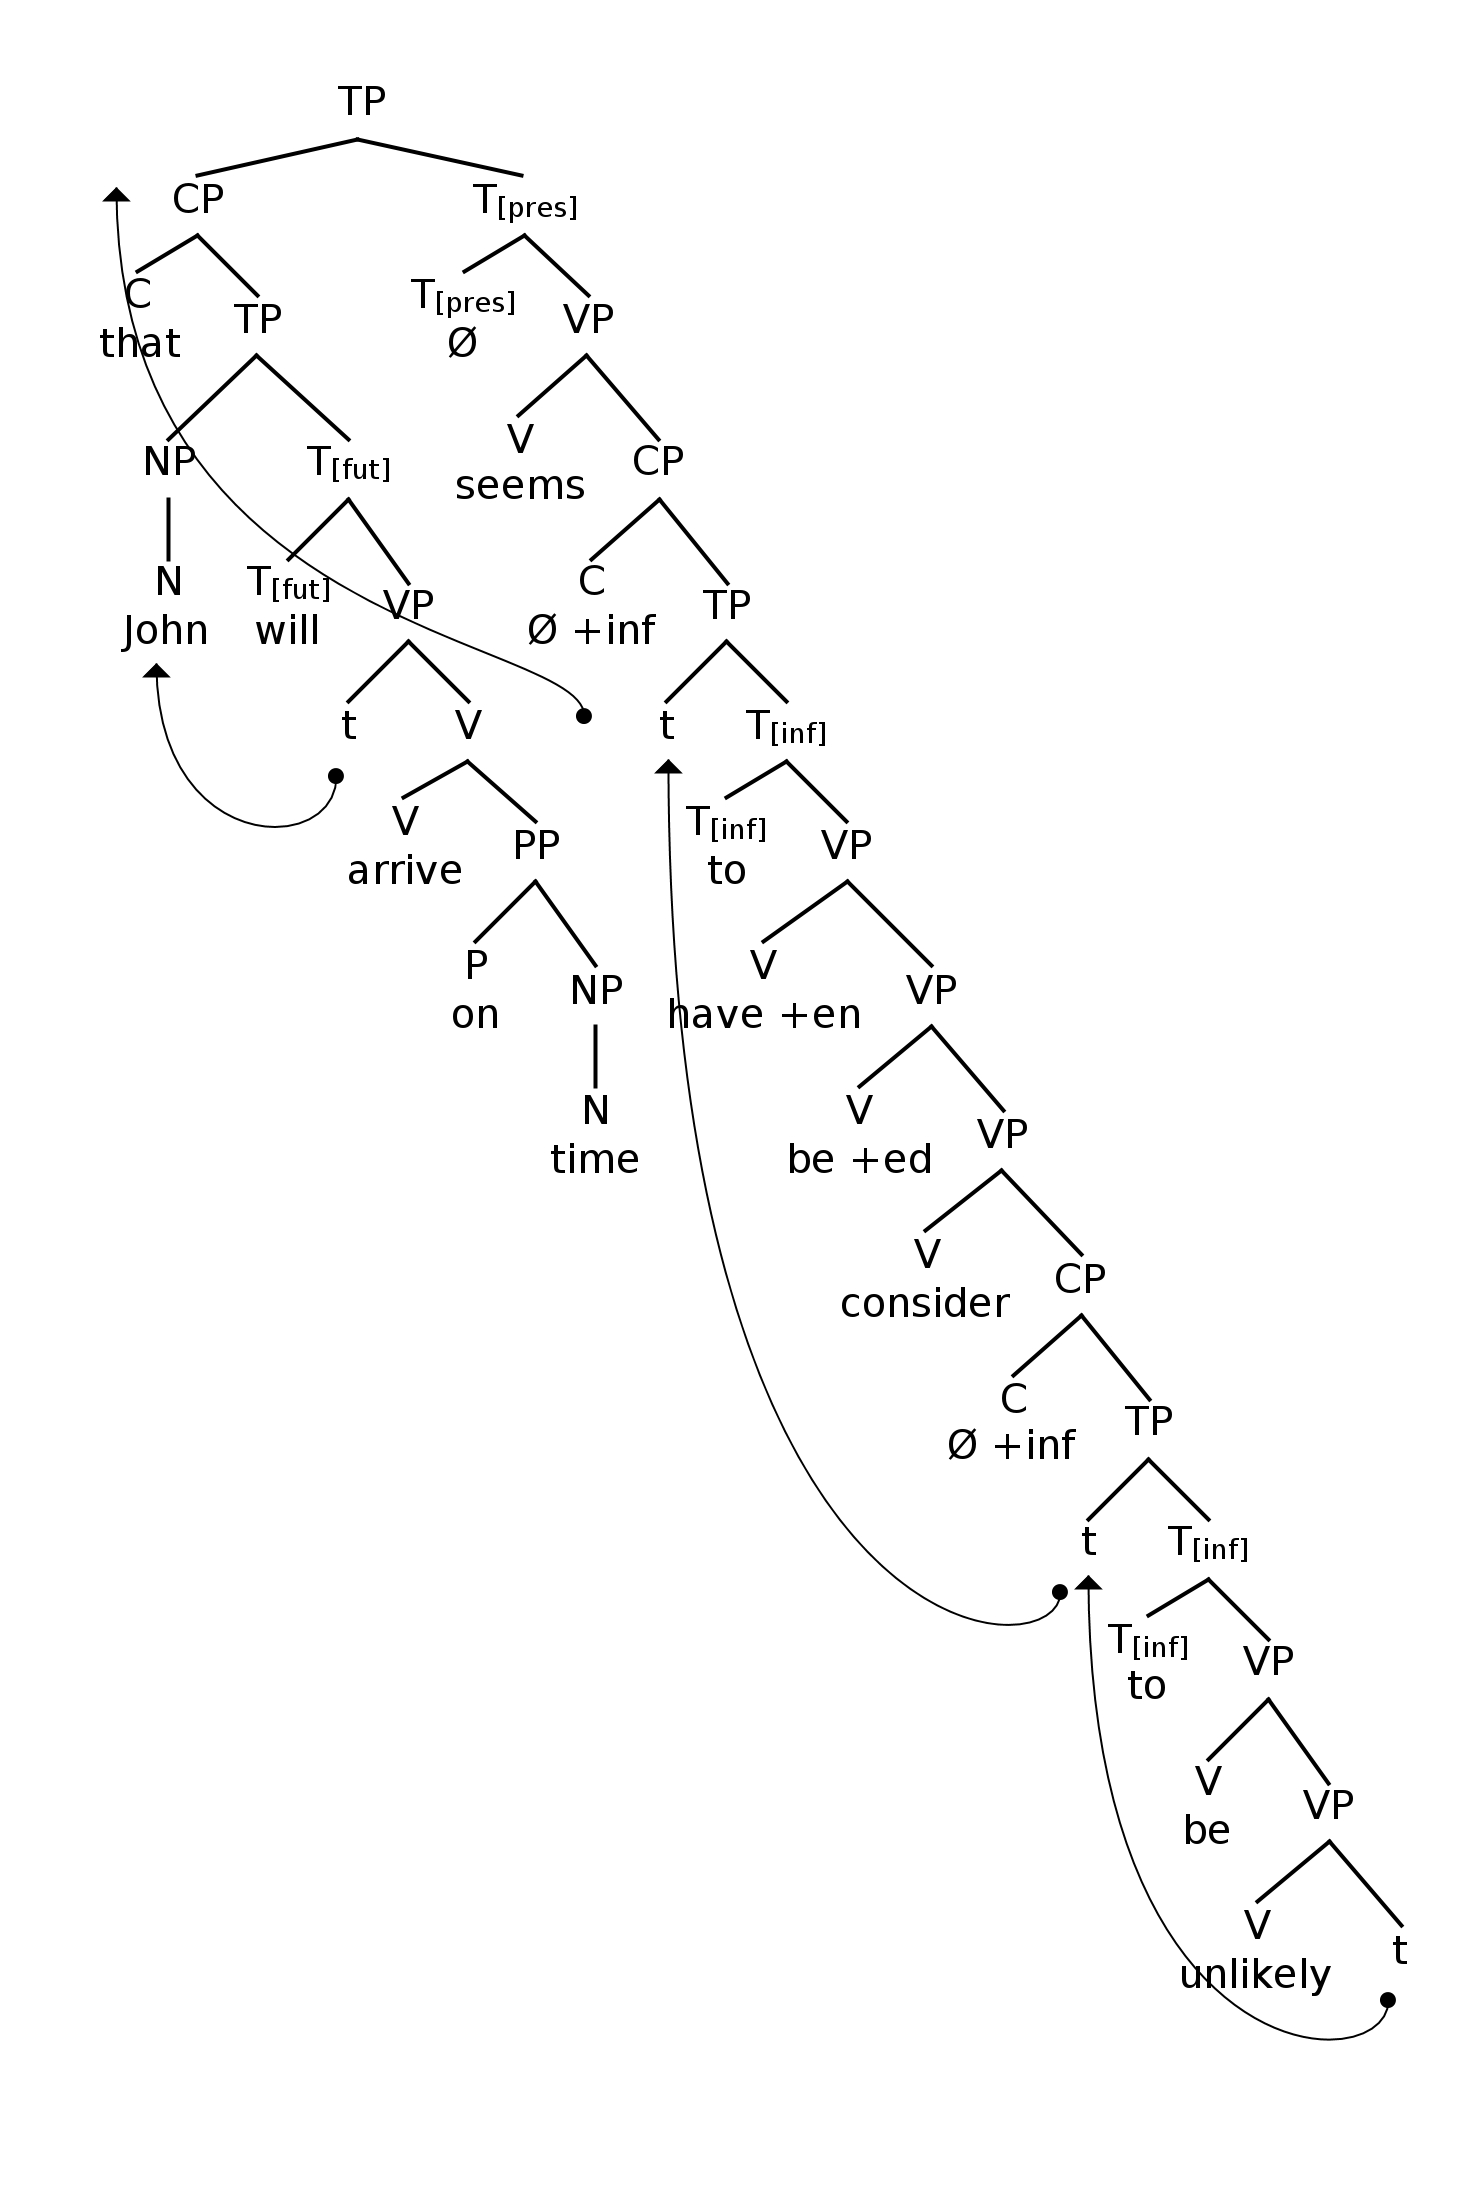
\includegraphics[height=7.8cm]{thatjohnwillarriveontimeseemstohavebeenconsideredtobeunlikely.jpg} }
\end{frame}


\begin{frame}[fragile]{Edge Features}
  Edge features probe for the first constituent available, or the last one to have uninterpretable features still unvalued
  \pause

  \only<2>{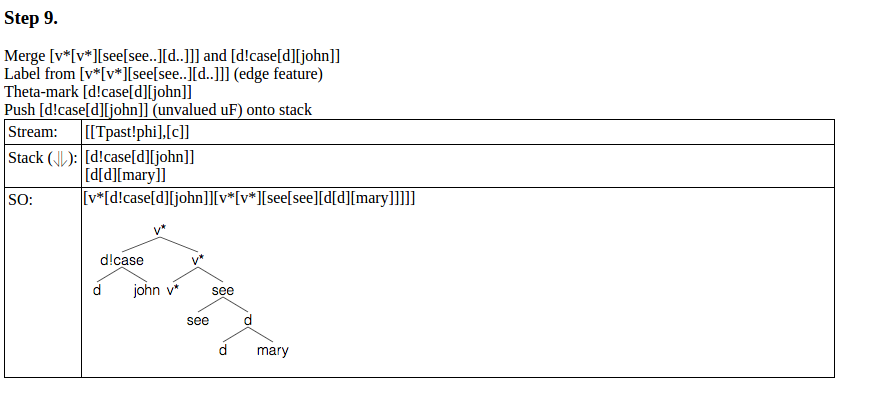
\includegraphics[height=5cm]{nocase1.png}}
  \only<3>{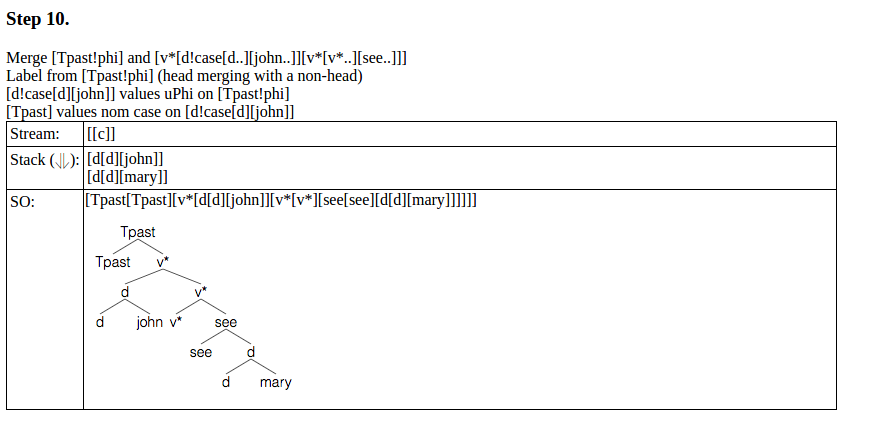
\includegraphics[height=5cm]{nocase2.png}}
  \only<4>{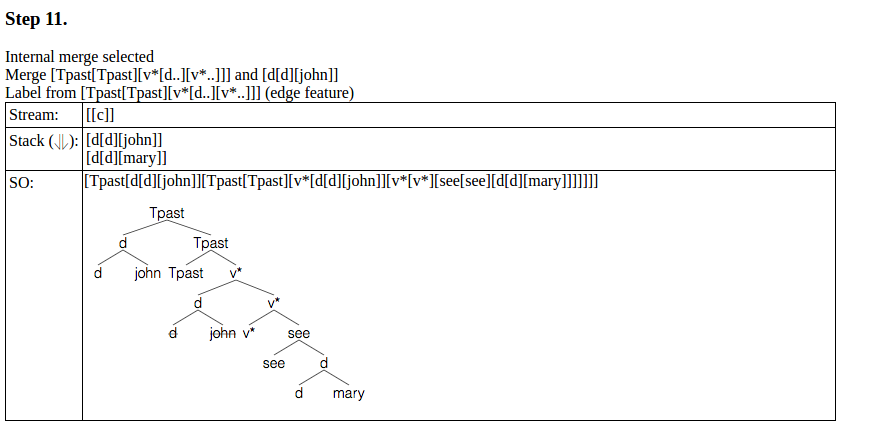
\includegraphics[height=5cm]{nocase3.png}}

  \onslide<2-4> This is realized in the Minimalist Machine with a stack onto which is pushed any item that does not have all its features valued.

\end{frame}








\begin{frame}[allowframebreaks]{References}

  \nocite{*}
  \bibliography{trevor-minimalist-machine}
  \bibliographystyle{abbrv}

\end{frame}

\end{document}
